\documentclass [a4paper,11pt]{article}
\usepackage{amssymb}
\usepackage{amsthm}
\usepackage[intlimits]{amsmath}
\usepackage[polish]{babel}
\usepackage[utf8]{inputenc}
\usepackage[T1]{fontenc}
\frenchspacing
\usepackage{indentfirst}
\usepackage{graphicx}
\usepackage{subfig}
\usepackage{mathptmx}
\usepackage{geometry}
\usepackage{wrapfig}
\usepackage{enumitem}
\usepackage{tabularx}

\title{Moduł Younga}
\author{Pęcak Tomasz, Bielech Maciej}

\begin{document}
	
	\renewcommand*{\figurename}{Rysunek} 
	\newgeometry{tmargin=2cm, bmargin=2cm, lmargin=2cm, rmargin=2cm}
	
	\linespread{1.5}
	\selectfont

	\begin{table}[]
		\centering
		\begin{tabular}{lllllll}
			\cline{1-6}
			\multicolumn{1}{|c|}{\begin{tabular}[c]{@{}c@{}}EAiIB\\ Informatyka\end{tabular}} & \multicolumn{2}{l|}{\begin{tabular}[c]{@{}l@{}}Pęcak Tomasz\\ Bielech Maciej\end{tabular}} & \multicolumn{1}{c|}{\begin{tabular}[c]{@{}c@{}}Rok\\ II\end{tabular}} & \multicolumn{1}{c|}{\begin{tabular}[c]{@{}c@{}}Grupa\\ 3a\end{tabular}} & \multicolumn{1}{c|}{\begin{tabular}[c]{@{}c@{}}Zespół\\ II\end{tabular}} &  \\ \cline{1-6}
			\multicolumn{1}{|c|}{\begin{tabular}[c]{@{}c@{}}Pracownia\\ FIZYCZNA\\ WFiIS AGH\end{tabular}} & \multicolumn{4}{l|}{\begin{tabular}[c]{@{}l@{}}Temat:\\ \textbf{Elektroliza} \end{tabular}} & 
			\multicolumn{1}{l|}{\begin{tabular}[c]{@{}l@{}}nr ćwiczenia:\\ 35\end{tabular}} &  \\ \cline{1-6}
			\multicolumn{1}{|l|}{\begin{tabular}[c]{@{}c@{}}Data wykonania:\\ 18.11.2017\end{tabular}} & \multicolumn{1}{c|}{\begin{tabular}[c]{@{}c@{}}Data oddania:\\ 21.11.2017\end{tabular}} & \multicolumn{1}{l|}{\begin{tabular}[c]{@{}l@{}}Zwrot do poprawki:\\ \phantom{data poprawki}\end{tabular}} & \multicolumn{1}{l|}{\begin{tabular}[c]{@{}l@{}}Data oddania:\\  \phantom{data oddania}\end{tabular}} & \multicolumn{1}{l|}{\begin{tabular}[c]{@{}l@{}}Data zaliczenia:\\  \phantom{data zaliczenia}\end{tabular}} & \multicolumn{1}{l|}{\begin{tabular}[c]{@{}l@{}}OCENA:\\ \phantom{ocena}\end{tabular}} &  \\ \cline{1-6} 
		\end{tabular}
	\end{table}
	 \hspace{5mm}

	\section{Wstęp}
	\section{Wykonanie ćwiczenia}
	\begin{figure}[!h]
		\centering
		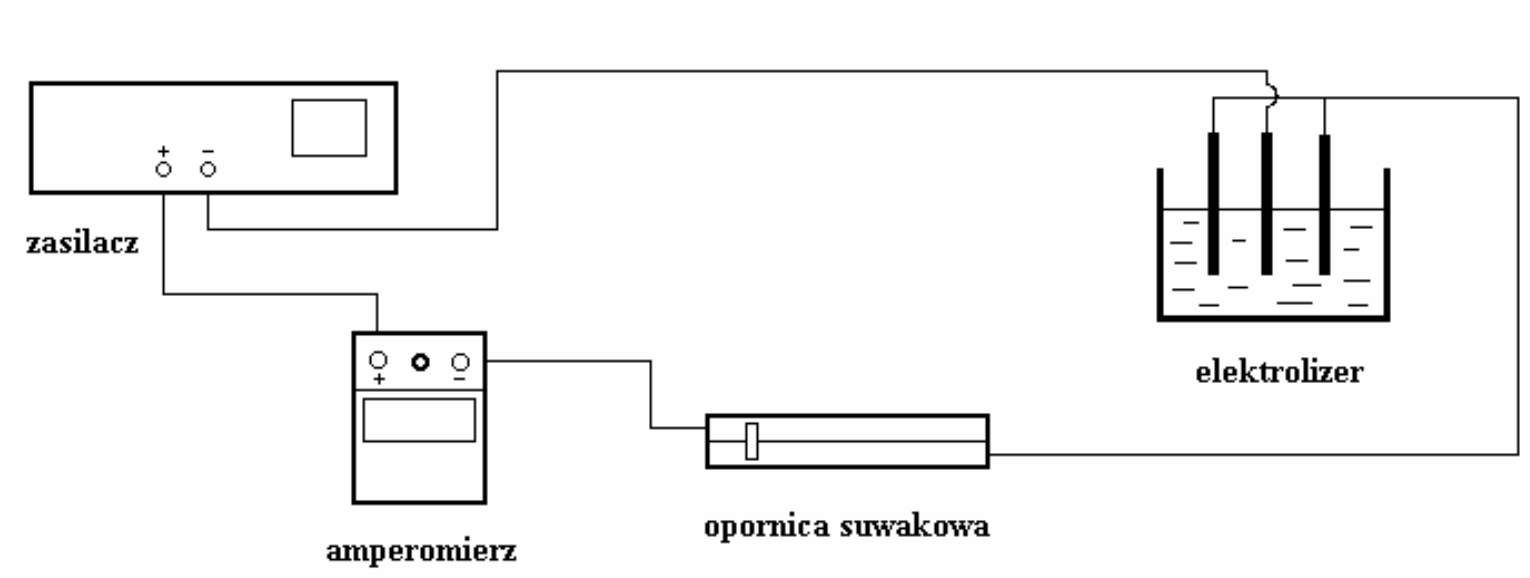
\includegraphics[width=0.6\textwidth]{uklad}
		\caption{Schemat zastosowanego obwodu elektrycznego}
		\label{fig:uklad}
	\end{figure}
	\begin{itemize}
		\item W pierwszym kroku, przy pomocy papieru ściernego, oczyszczono katodę i anody. Następnie zostały one przemyte bieżącą wodą i opłukane wodą destylowaną. Po czym, przy pomocy suszarki, dokładnie je wysuszono.
		
		\item W kolejnym kroku, po ostygnieciu elektrod, dokonano pomiaru ich mas.
		
		\item Następnie złożono układ zgodnie ze schematem(\ref{fig:uklad}). Po sprawdzeniu obowdu, uruchomiono zasilacz przy jednoczesnym rozpoczęciu pomiaru czasu.
		W czasie trwania elektrolizy dbano o utrzymanie stałego natężenia($0,5$ A).
		
		\item  Po upływie 30 minut wyłączono zasilanie i powtórnie zważono katodę i anody.
	\end{itemize}

	
	\section{Opracowanie danych pomiarowych}\label{sec:opr}
	\subsection{Pomiary i ich niepewności.}
	\begin{itemize}
		\item Masa
			\begin{center}
			\begin{tabular}{p{0.1\linewidth}|p{0.13\linewidth}|p{0.15\linewidth}|p{0.1\linewidth}}
				&masa przed elektrolizą[g]&masa po elektrolizie[g]& różnica[g]\\
				\hline
				katoda&$75.448$&$75.744$&$0.296$ \\
				\hline
				anody &$201.460$&$201.170$&$0.290$ \\
			\end{tabular} 	
		\end{center}
		Ze względu na zanieczyszczenia oraz ryzyko niedokładnego wysuszenia elektrod, przy pomiarach masy przyjeliśmy niepewność większą od niepewności znamionowej użytej wagi($\Delta m=0.001$ g) równą $u(m)=0.003$. 
		
		\item Czas $ t=1800$s
		
		Niepewnośc zmierzonego czasu została przez nas pominięta, ze względu na niezauważalny wpływ na wynik($\approx0.05$ \%). W dalszych obliczeniach nie uzwględniamy czasu 
		przy wyznaczaniu niepewności roszerzonych poszczególnych wielkości.
		
		\item Natężenie $I=0.5$A
		
		Niepewność natężenia wyznaczamy ze wzoru:
	\end{itemize}
	\begin{equation}
	\label{eq:amper}
	u(I) = \frac{\text{klasa amperomierza} \cdot \text{zakres}}{100} = 3,75 \cdot 10^{-3} [A].
	\end{equation}

 	\begin{equation}
 	k = \frac{m}{I t} = \frac{296 \cdot 10^{-3}}{0,5 \cdot 1,8 \cdot 10^3} \approx 3,288\cdot 10^{-4} \left[  \frac{g}{A \cdot s}\right] 
 	\label{k_obliczone} 
 	\end{equation}
 	

 	\begin{equation}
 	F = \frac{\mu}{w k} = \frac{63,58 }{2 \cdot 3,219 \cdot 10^{-4}} \approx 96598  \left[  \frac{C}{mol}\right] 
 	\label{F_obliczone} 
 	\end{equation}
 	

 	\begin{equation}
 	e = \frac{F}{N_A} = \frac{96598 }{6,02 \cdot 10^{23}} \approx 1,604 \cdot 10^{-19}   \left[  C \right] 
 	\label{e_obliczone} 
 	\end{equation}
 	
 	\section{Obliczanie niepewności pomiarowej}
 	

 	

 	\begin{equation}
 	\frac{u(k)}{k} = \sqrt{\left[\frac{u(m)}{m} \right]^2 + \left[\frac{u(I)}{I} \right]^2 } = \sqrt{\left[\frac{ 0,003}{0,296} \right]^2 + \left[\frac{0,00375}{0,5} \right]^2 } \approx 0,0126
 	\end{equation}
 	
 	\begin{equation}
 	u(k) = \frac{u(k)}{k} \cdot k =  0,0126 \cdot 0,3288 \cdot 10^{-3} \approx 0,0041 \cdot 10^{-3}  \left[  \frac{g}{A \cdot s}\right] 
 	\end{equation}
 	

 	\begin{equation}
 	\frac{u(F)}{F} = \sqrt{\left[\frac{u(\mu)}{\mu} \right]^2 + \left[\frac{u(k)}{k} \right]^2 } = \sqrt{\left[\frac{u(k)}{k} \right]^2 } = \frac{u(k)}{k}  
 	\end{equation}
 	
 	\begin{equation}
 	u(F) = F \frac{u(k)}{k}  =  96597  \cdot  0,0126 \approx 1217  \left[  \frac{C}{mol}\right] 
 	\end{equation}
 	\begin{equation}
 	\frac{u(e)}{e}=\sqrt{\left[\frac{u(F)}{F}\right]^2} =  \frac{u(F)}{F} =  \frac{u(k)}{k}
 	\end{equation}
 	
 	\begin{equation}
 	u(e) = e \frac{u(k)}{k}  =  1,604 \cdot 10^{-19}  \cdot  0,0126 \approx 0,0202 \cdot 10^{-19} [C] 
 	\end{equation}
 	
	
	\subsection{Opracowanie danych.}\label{sec:drm}
	\begin{enumerate}[label=\alph*)]
		
		\item Analiza błędów.
		
		Stwierdzono wystąpienie błędów grubych, które wyraźnie odstają od średniej. Zaznaczono je w tabelkach kolorem czerwonym.
		
		\item Obliczenie wartości rezystancji połączeń szeregowego, równoległego i mieszanego korzystając z wyników pomiarów $R_1$, $R_2$ i $R_3$ i ich niepewności.
		

		
		Niepewności wyliczenia rezystancji zastępczych obliczone zostały z wykorzystaniem prawa przenoszenia niepewności za pomocą następujących wzorów:

		

	
	\end{enumerate}
	
	\section{Podsumowanie}
	\begin{tabular}{|c|c|c|c|c|c|}
		\hline  & wartość tablicowa  & wartość wyznaczona& różnica & niepewność  & niepewność względna [\%]  \\ 
		\hline $k \left[  \frac{mg}{A \cdot s}\right]$ & 0,3294  & 0,3289  & 0,0005  & 0,0041  & 1,26  \\ 
		\hline $F \left[  \frac{C}{mol}\right]$ & 96500 & 96597  & 97  & 1218  & 1,26  \\ 
		\hline $e [10^{-19} C]$ & 1,6022   & 1,604    & 0,0018    & 0,0202   & 1,26  \\ 
		\hline 
	\end{tabular} 
\vspace{1em}



\end{document}